% A bar chart (grid lines with tick labels, filled bars with value labels)
% next to a paragraph: no table must be detected.
\documentclass[a4paper,10pt]{article}
\usepackage[utf8]{inputenc}
\usepackage[T1]{fontenc}
\usepackage{lmodern}
\usepackage{tikz}
\pagestyle{empty}
\setlength{\parindent}{0pt}
\begin{document}
Prihodi po segmentima u milijunima eura.

\vspace{1em}
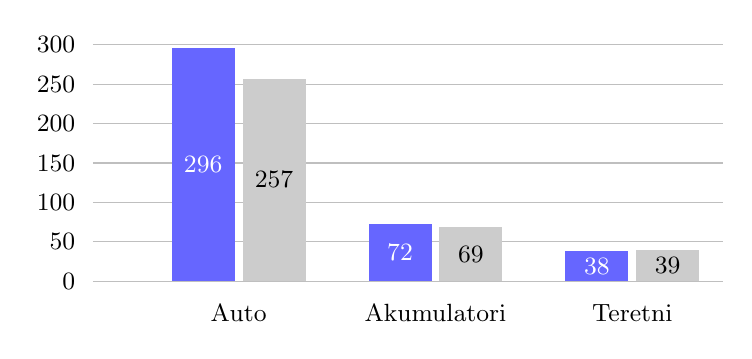
\begin{tikzpicture}[x=1cm,y=0.5cm,font=\small]
  \foreach \v in {0,50,100,150,200,250,300} {
    \draw[gray!50] (0,\v/50) -- (8,\v/50);
    \node[anchor=east] at (-0.1,\v/50) {\v};
  }
  \foreach \x/\a/\b in {1/296/257, 3.5/72/69, 6/38/39} {
    \fill[blue!60] (\x,0) rectangle (\x+0.8,\a/50);
    \fill[gray!40] (\x+0.9,0) rectangle (\x+1.7,\b/50);
    \node[white] at (\x+0.4,\a/100) {\a};
    \node at (\x+1.3,\b/100) {\b};
  }
  \node at (1.85,-0.8) {Auto};
  \node at (4.35,-0.8) {Akumulatori};
  \node at (6.85,-0.8) {Teretni};
\end{tikzpicture}

\vspace{1em}
Prihodi ostvareni poslovanjem u segmentu autodijelova čine najznačajniji udio u
ukupno ostvarenim prihodima od prodaje Grupe.
\end{document}
